Das Spiel Heyawake (japanisch \begin{CJK}{UTF8}{min}へやわけ\end{CJK},
``Zimmeraufteilung'', \begin{CJK}{UTF8}{min}わけ\end{CJK} kann aber auch
als \begin{CJK}{UTF8}{min}訳\end{CJK}
mit der Bedeutung ``Schlussfolgerung'' gelesen werden)
wird auf einem $n\times m$-Spielfeld gespielt, das durch dicke Linien in
Rechtecke aufgeteilt ist, die Zimmer genannt werden:
\begin{center}
\def\punkt#1#2{ ({0.8*(#1)},{0.8*(#2)}) }
\def\feld{
	\foreach \i in {1,...,4}{
		\draw \punkt{\i}{0} -- \punkt{\i}{5};
		\draw \punkt{0}{\i} -- \punkt{5}{\i};
	}
	\draw[line width=2.1pt] \punkt{0}{0} rectangle \punkt{1}{3};
	\draw[line width=2.1pt] \punkt{1}{0} rectangle \punkt{2}{3};
	\draw[line width=2.1pt] \punkt{2}{0} rectangle \punkt{4}{4};
	\draw[line width=2.1pt] \punkt{4}{0} rectangle \punkt{5}{4};
	\draw[line width=2.1pt] \punkt{0}{3} rectangle \punkt{2}{5};
	\draw[line width=2.1pt] \punkt{2}{4} rectangle \punkt{4}{5};
	\draw[line width=2.1pt] \punkt{4}{4} rectangle \punkt{5}{5};
	\node at \punkt{0.5}{4.5} {\large $1$};
	\node at \punkt{0.5}{2.5} {\large $2$};
	\node at \punkt{2.5}{3.5} {\large $4$};
}
\def\schwarz#1#2{
	\fill[color=gray!40] \punkt{#1}{#2} rectangle \punkt{#1+1}{#2+1};
}
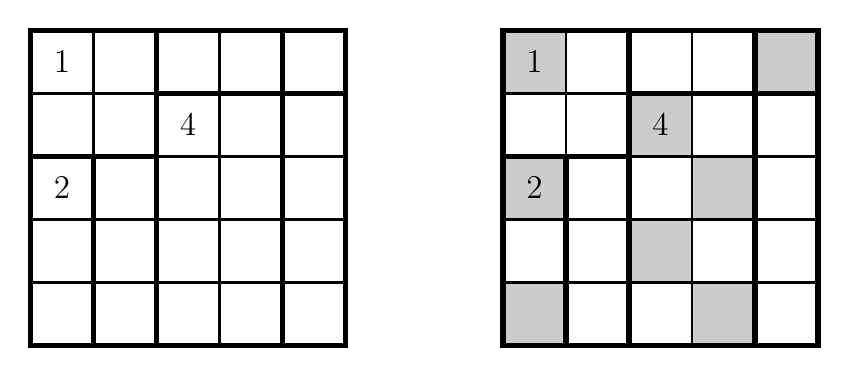
\begin{tikzpicture}[>=latex,thick]
\begin{scope}[xshift=-3cm]
\feld
\end{scope}
\begin{scope}[xshift=3cm]
\schwarz{0}{0}
\schwarz{0}{2}
\schwarz{0}{4}
\schwarz{2}{1}
\schwarz{2}{3}
\schwarz{3}{0}
\schwarz{3}{2}
\schwarz{4}{4}
\feld
\end{scope}
\end{tikzpicture}
\end{center}
Der Spieler muss einzelne Felder schwarz einfärben wie in der Abbildung
rechts, dabei aber folgende Regeln einhalten:
\begin{enumerate}
\item
Eingefärbte Felder dürfen sich nicht enlang einer Kante berühren.
\item
Alle weissen Felder müssen untereinander verbunden sein.
\item
Falls in einem Zimmer eine Zahl eingetragen ist, müssen in diesem
Zimmer soviele Felder einfärbt werden, wie die Zahl angibt.
\item
Ein Zimmer ohne Zahl darf beliebig viele eingefärbte Felder enthalten.
\item
Eine horizontale oder vertikale Linie von benachbarten weissen
Feldern darf sich höchstens über zwei Zimmer erstrecken oder
anders ausgedrückt: eine solche Linie, die drei oder mehr Zimmer
verbindet, ist verboten.
\end{enumerate}
Kann eine nichtdeterministische Turing-Maschine in polynomieller
Zeit entscheiden, ob ein Heyawake-Rätsel lösbar ist?

\thema{NP}
\thema{polynomieller Verifizierer}

\begin{loesung}
Das Problem ist sicher entscheidbar, indem man alle $2^{nm}$ Möglichkeiten
durchprobiert.
Es ist auch in der Klasse NP, wenn es einen polynomiellen Verifizierer
gibt.
Als Lösungszertifikat werden die alle einfärbten Felder benötigt.

Der Verfikationsalgorithums muss folgende Prüfungen durchführen:
\begin{center}
\renewcommand{\arraystretch}{1.2}
\begin{tabular}{|c|p{12cm}|>{$}c<{$}|}
\hline
Schritt&Verifikation&\text{Aufwand}\raisebox{3pt}{\strut}\\
\hline
1&\strut
Für jedes einfärbte Feld prüfe, ob die horizontalen und
vertikalen Nachbarfelder nicht schwarz sind\strut
&O(nm) \mathstrut\\
2&\strut
Beginne beim ersten weissen Feld und färbe alle weissen Nachbarfelder
rot ein.
Wenn ein weisses Feld übrig bleibt, liegt keine Lösung vor.\strut
&O(nm) \mathstrut\\
3&\strut
Für jedes Feld, welches eine Zahl enthält, zähle die schwarzen
Felder im gleichen Zimmer und prüfe, ob sie mit der Zahl übereinstimmt.\strut
&O(n^2m^2)\mathstrut\\
4&\strut
Für jedes weisse Feld, folge horizontal und vertikal den weissen
Feldern bis zu einem schwarzen Feld oder bis zum Spielfeldrand.
Wenn dabei mehr als 2 Zimmerwände gekreuzt werden, liegt keine Lösung
vor.\strut
&O(n^2m+nm^2)\mathstrut\\
\hline
&Total&O(n^2m^2)\mathstrut \\
\hline
\end{tabular}
\end{center}
Die Verifikation ist offenbar in polynomieller Zeit möglich.
Damit ist gezeigt, dass Heyawake in NP ist.

Die Verifikation könnten noch etwas effizienter gestaltet werden, wenn
alle weissen Felder, die mit dem ersten weissen Feld verbunden sind,
rot eingefärbt werden.
Dann muss im zweiten Schritt nur geprüft werden, ob alle nicht
schwarzen Nachbarfelder die gleiche Farbe haben.

Ein Heywake Rätsel ist ein polynomielles Ausfüllrätsel.
Die im Verifikationsalgorithmus formulierten Schritte sind
als Regeln formuliert, die für eine Feld des Spielfeldes erfüllt
sein müssen.
Sie können offensichtlich in polynomieller Zeit ausgewertet werden.
Als polynomielles Ausfüllrätsel ist Heyawake automatisch in NP.
\end{loesung}

\begin{diskussion}
Heyawake wurde 1992 von Nikoli veröffentlich.
Markus Holzer und Oliver Ruepp haben gezeigt, dass Heyawake
NP-vollständig ist: {\em The troubles of interior design --- complexity
analysis of the game Heywake},
Proceedings, 4th International Converence on Fun with Algorithms,
Lecture Notes in Computer Science 4475, Springer-Verlag, Berlin/Heidelberg
2007,
\url{https://doi.org/10.107/978-3-540-72914-3_18}
\end{diskussion}

\begin{bewertung}
Entscheidbarkeit ({\bf E}) 1 Punkt,
Prinzip Verifizierer ({\bf V}) 1 Punkt,
Zertifikat spezifiziert ({\bf Z}) 1 Punkt,
Laufzeitschätzung ({\bf L}) 2 Punkte,
Schlussfolgerung polynomieller Verifizierer ({\bf S}) 1 Punkt.
\end{bewertung}

